\documentclass[11pt]{article}
\usepackage[margin=1in]{geometry}
\usepackage{amsmath,amssymb,amsthm}
\usepackage{graphicx}
\usepackage{hyperref}

\newtheorem{lemma}{Lemma}
\newtheorem{theorem}{Theorem}
\newtheorem{corollary}{Corollary}

\title{Predictive Geometric Control of Quantum\\
Dynamics via Spectral Curvature Functional\\
$\Lambda(t)$}
\author{R. J. Mathews\\
Independent Researcher\\
\texttt{rjmathews@getqore.ai}}
\date{November 2025 --- revised July 2026 (v2: simulation section added; Landau--Zener exponent normalization corrected)}

\begin{document}
\maketitle

\begin{abstract}
Non-adiabatic transitions remain a dominant source of leakage and decoherence in electrically controlled qubits, including semiconductor spin qubits driven through avoided crossings via Landau--Zener--St\"uckelberg--Majorana (LZSM) interference. Conventional control methods are reactive: leakage is measured only after an error has already occurred. We introduce a predictive control framework based on a \emph{spectral curvature functional} $\Lambda(t)$, defined as the operator norm of the commutator between the instantaneous generator of evolution and its time derivative. For a two-level quantum system governed by a time-dependent Hamiltonian $\mathcal{H}(t) = \frac{\hbar}{2}(\Delta(t)\sigma_z + \Omega \sigma_x)$ with constant coupling $\Omega$, we derive an exact identity
\[
    \Lambda(t) = \frac{1}{2}\Omega |\dot{\Delta}(t)|.
\]
At the gap minimum $t^*$, the Landau--Zener transition probability satisfies
\[
    P_{LZ} \approx \exp\left(-\frac{\pi\Omega^3}{4\Lambda(t^*)}\right),
\]
establishing a direct, pointwise control law: minimizing peak curvature at the avoided crossing exponentially suppresses leakage. This is complemented by a frequency-domain analysis showing that peak curvature is bounded by the spectral first moment $\int |\omega| |\hat{\Delta}(\omega)|\, d\omega$, providing a rigorous low-pass design rule. We present a predictive feedback loop that enforces $\Lambda(t) \le \alpha_{\mathrm{crit}}$ during gate operation. Time-dependent Schr\"odinger simulations of LZSM sweeps (90 runs across linear, tanh, and Gaussian-flattened detuning schedules) confirm the pointwise law: measured leakage collapses onto a single function of the peak curvature $\Lambda(t^*)$, matching the displayed exponent constant with fitted slope $1.003$, and a curvature-flattened waveform reduces measured leakage by factors of $8$ to $5.7\times 10^{3}$ relative to a naive linear ramp at equal sweep range and equal total time, without requiring counter-diabatic fields or full Hamiltonian inversion. This work provides a simple geometric precursor for non-adiabatic transitions and a practical control strategy compatible with existing pulse-generation hardware.
\end{abstract}

%=============================================================================
\section{Introduction}
%=============================================================================

Electrically controlled qubits, particularly semiconductor spin qubits, frequently rely on avoided crossings to implement state transfer or phase accumulation. Leakage during these crossings is typically modeled by the Landau--Zener (LZ) formula, producing a transition probability
\begin{equation}
    P_{LZ} \approx \exp\left(-\frac{\pi\Omega^2}{2\nu}\right),
    \label{eq:lz-standard}
\end{equation}
where $\Omega$ is the transverse coupling and $\nu = |\dot{\Delta}(t^*)|$ is the detuning sweep rate at the minimum gap.\footnote{\textit{Revision note (July 2026):} earlier drafts of this paper printed Eq.~\eqref{eq:lz-standard} --- and consequently Eqs.~\eqref{eq:lz-curvature} and \eqref{eq:lz-combined}--\eqref{eq:bandlimit-lower} --- without the factor of two in the exponent's denominator, overstating the leakage suppression by a factor of two in the exponent. The time-dependent Schr\"odinger simulations of Section~5 identified the discrepancy (fitted exponent slope $1.003$ against the standard normalization), and this revision propagates the standard Landau--Zener constant throughout. Lemma~1 and the pointwise control law are unaffected.} Existing control approaches measure leakage only after it has occurred, requiring repeated calibration or counter-diabatic corrections.

We propose a predictive control parameter: the \emph{spectral curvature functional} $\Lambda(t)$. This observable produces a precursor signal for imminent leakage and yields a direct control objective: constrain $\Lambda$ near the avoided crossing to suppress $P_{LZ}$ in real time.

%=============================================================================
\section{Mathematical Framework}
%=============================================================================

Consider a two-level Hamiltonian
\begin{equation}
    \mathcal{H}(t) = \frac{\hbar}{2}(\Delta(t)\sigma_z + \Omega\sigma_x),
    \label{eq:hamiltonian}
\end{equation}
with $\Omega$ constant and $\Delta(t)$ a control waveform. Define the instantaneous generator
\[
    B(t) = \frac{\mathcal{H}(t)}{\hbar}
\]
and the \emph{curvature functional}
\begin{equation}
    \Lambda(t) = \|[B(t), \dot{B}(t)]\|,
    \label{eq:curvature-def}
\end{equation}
where $\|\cdot\|$ denotes the operator norm. Non-zero $\Lambda$ indicates that the instantaneous plane of rotation is changing, signaling non-adiabatic driving.

\subsection{Lemma 1: Curvature--Sweep Identity}

\begin{lemma}
For the Hamiltonian in Eq.~\eqref{eq:hamiltonian} with constant $\Omega$, the curvature functional satisfies
\begin{equation}
    \Lambda(t) = \frac{1}{2}\Omega|\dot{\Delta}(t)|.
    \label{eq:curvature-identity}
\end{equation}
\end{lemma}

\begin{proof}
We compute
\[
    B(t) = \frac{1}{2}(\Delta(t)\sigma_z + \Omega\sigma_x), \quad \dot{B}(t) = \frac{\dot{\Delta}(t)}{2}\sigma_z.
\]
Commuting gives
\[
    [B(t), \dot{B}(t)] = \frac{\Omega\dot{\Delta}(t)}{4}[\sigma_x, \sigma_z] = \frac{\Omega\dot{\Delta}(t)}{4}(-2i\sigma_y) = -\frac{i\Omega\dot{\Delta}}{2}\sigma_y.
\]
Taking the standard operator norm $\|\sigma_y\| = 1$, this yields $\Lambda(t) = \left\|-\frac{i\Omega\dot{\Delta}}{2}\sigma_y\right\| = \frac{1}{2}\Omega|\dot{\Delta}(t)|$.
\end{proof}

\subsection{Lemma 2: Peak Curvature Controls Leakage}

Let $t^*$ denote the minimum gap, i.e.\ $\Delta(t^*) \approx 0$. From Eq.~\eqref{eq:lz-standard} and $\nu = |\dot{\Delta}(t^*)| = 2\Lambda(t^*)/\Omega$ (from Lemma~1), we obtain:

\begin{lemma}
The Landau--Zener transition probability is expressible directly in terms of the curvature at the gap minimum:
\begin{equation}
    P_{LZ} \approx \exp\left(-\frac{\pi\Omega^3}{4\Lambda(t^*)}\right).
    \label{eq:lz-curvature}
\end{equation}
\end{lemma}

Equation~\eqref{eq:lz-curvature} establishes a pointwise, predictive control law: minimizing $\Lambda(t^*)$ exponentially suppresses leakage.

%=============================================================================
\section{Frequency--Domain Analysis of the Curvature Functional}
%=============================================================================

In this section we derive a frequency--domain bound on the peak curvature $\Lambda(t^*)$. Throughout, we assume $\Delta(t)$ is a pulse with $\dot{\Delta} \in L^1(\mathbb{R})$ so that all Fourier transforms are well-defined. While the transform definitions below assume causality for simplicity, the core time-domain results (Lemmas~1, 2) hold generally. The Fourier transform is defined as $\hat{f}(\omega) \equiv \int_{-\infty}^{\infty} f(t) e^{-i\omega t}\, dt$.

\subsection{Spectral Moment Bound on Peak Curvature}

The next result converts the pointwise slope $|\dot{\Delta}(t^*)|$ into an inequality involving a spectral first moment of the control pulse. It uses only the triangle inequality for the inverse Fourier transform and requires no bandlimit assumption.

\begin{theorem}[Spectral moment bound on peak curvature]
Suppose $\hat{\Delta} \in L^1(\mathbb{R}, (1 + |\omega|)\, d\omega)$. Then for every $t$,
\begin{equation}
    |\dot{\Delta}(t)| \le \frac{1}{2\pi} \int_{-\infty}^{\infty} |\omega| |\hat{\Delta}(\omega)|\, d\omega.
    \label{eq:slope-bound}
\end{equation}
Consequently, the peak curvature at the avoided crossing $t^*$ satisfies
\begin{equation}
    \Lambda(t^*) \le \frac{\Omega}{4\pi} \int_{-\infty}^{\infty} |\omega| |\hat{\Delta}(\omega)|\, d\omega.
    \label{eq:curvature-bound}
\end{equation}
\end{theorem}

\begin{proof}
By Fourier inversion,
\[
    \dot{\Delta}(t) = \frac{1}{2\pi} \int_{-\infty}^{\infty} (i\omega) \hat{\Delta}(\omega) e^{i\omega t}\, d\omega.
\]
Taking absolute values and applying the triangle inequality yields
\[
    |\dot{\Delta}(t)| \le \frac{1}{2\pi} \int_{-\infty}^{\infty} |\omega| |\hat{\Delta}(\omega)|\, d\omega,
\]
which is~\eqref{eq:slope-bound}. Multiplying by $\Omega/2$ (from Lemma~1) gives~\eqref{eq:curvature-bound}.
\end{proof}

\begin{corollary}[Low-pass design rule]
If $\hat{\Delta}$ is supported in $[-\omega_c, \omega_c]$, then
\begin{equation}
    \Lambda(t^*) \le \frac{\Omega \omega_c}{4\pi} \int_{-\infty}^{\infty} |\hat{\Delta}(\omega)|\, d\omega.
    \label{eq:bandlimit-bound}
\end{equation}
Equivalently, for fixed $\|\hat{\Delta}\|_{L^1}$, reducing the bandwidth $\omega_c$ reduces an a priori upper bound on the peak curvature.
\end{corollary}

\begin{proof}
Under the bandlimit, $|\omega| \le \omega_c$ on the support of $\hat{\Delta}$, giving
\[
    \int |\omega| |\hat{\Delta}(\omega)|\, d\omega \le \omega_c \int |\hat{\Delta}(\omega)|\, d\omega.
\]
Apply Theorem~1.
\end{proof}

\subsection{Consequences for Landau--Zener Leakage}

Let $\nu^* \equiv |\dot{\Delta}(t^*)|$ be the local sweep rate at the gap minimum. The Landau--Zener formula~\cite{landau1932,zener1932,stueckelberg1932,majorana1932} gives
\begin{equation}
    P_{LZ} \approx \exp\left(-\frac{\pi\Omega^2}{2\nu^*}\right) = \exp\left(-\frac{\pi\Omega^3}{4\Lambda(t^*)}\right).
    \label{eq:lz-combined}
\end{equation}
Combining~\eqref{eq:lz-combined} with~\eqref{eq:curvature-bound} yields the \emph{spectral lower bound}
\begin{equation}
    P_{LZ} \ge \exp\left(-\frac{\pi\Omega^{3}/4}{\frac{\Omega}{4\pi}\int |\omega| |\hat{\Delta}(\omega)|\, d\omega}\right) = \exp\left(-\frac{\pi^2\Omega^2}{\int_{-\infty}^{\infty} |\omega| |\hat{\Delta}(\omega)|\, d\omega}\right).
    \label{eq:spectral-lower-bound}
\end{equation}

In particular, for a fixed spectral moment $\int |\omega| |\hat{\Delta}|$, no control schedule can drive $P_{LZ}$ below the right-hand side of~\eqref{eq:spectral-lower-bound}. Under the bandlimit of Corollary~1 we also obtain
\begin{equation}
    P_{LZ} \ge \exp\left(-\frac{\pi^2\Omega^2}{\omega_c \|\hat{\Delta}\|_{L^1}}\right).
    \label{eq:bandlimit-lower}
\end{equation}

\textbf{Remarks.} (i) The bounds~\eqref{eq:spectral-lower-bound}--\eqref{eq:bandlimit-lower} are lower bounds on the achievable leakage, consistent with the monotonicity of $P_{LZ}$ in $\nu^*$. (ii) Unlike global time--domain heuristics (e.g.\ total variation), the spectral moment $\int |\omega| |\hat{\Delta}|$ controls \emph{all} pointwise slopes via~\eqref{eq:slope-bound}, with no averaging. (iii) Stronger bounds follow by adding smoothness constraints, e.g.\ $|\ddot{\Delta}| \le L$ on a neighborhood of $t^*$ (yielding windowed variants using local spectral content). We omit these for brevity.

\subsection{Design Implications}

The frequency--domain identities and bounds justify curvature--constrained waveform design:

\begin{enumerate}
    \item \textbf{Low spectral first moment} $\int |\omega| |\hat{\Delta}| \Rightarrow$ smaller a priori bound on $\Lambda(t^*)$.
    \item \textbf{Bandlimit or low-pass shaping} (Corollary~1) $\Rightarrow$ explicit handle on the curvature peak via $\omega_c$ and $\|\hat{\Delta}\|_{L^1}$.
    \item \textbf{Predictive control objective:} enforce $\Lambda(t) \le \alpha_{\mathrm{crit}}$ near $t^*$ and co-design the pulse to minimize the spectral moment, thereby reducing the fundamental leakage lower bound~\eqref{eq:spectral-lower-bound}.
\end{enumerate}

%=============================================================================
\section{Predictive Control Loop}
%=============================================================================

The control objective is to enforce
\[
    \Lambda(t) \le \alpha_{\mathrm{crit}}
\]
for $t$ near $t^*$. This is implemented as a feedback loop:

\begin{itemize}
    \item Measure or estimate $\Delta(t)$ in real time.
    \item Compute $\Lambda(t)$ via Eq.~\eqref{eq:curvature-identity}.
    \item If $\Lambda > \alpha_{\mathrm{crit}}$, adjust the waveform slope (reduce $|\dot{\Delta}|$).
\end{itemize}

\subsection{Pseudocode}

\begin{verbatim}
Initialize waveform Delta(t)
for each timestep t:
    measure or estimate Delta
    compute Lambda = 0.5 * Omega * abs(dDelta/dt)
    if Lambda > alpha_crit:
        reduce slope of Delta(t)
    update DAC output
end
\end{verbatim}

\subsection{Implementation Considerations}

We note that a practical, real-time implementation of this loop faces significant engineering challenges, including measurement back-action, system latency, and finite control bandwidth. This paper presents the theoretical control principle; a hardware demonstration would require translating this objective into an open-loop optimized pulse (using Section~3) or a closed-loop controller that respects these physical constraints, possibly by using model-based estimation rather than direct, disruptive measurement.

%=============================================================================
\section{Simulation}
\label{sec:simulation}
%=============================================================================

\textbf{Protocol.} We integrate the time-dependent Schr\"odinger equation $i\dot{\psi} = B(t)\psi$ for the generator of Eq.~\eqref{eq:hamiltonian} (Dormand--Prince DOP853, relative tolerance $10^{-11}$, absolute tolerance $10^{-13}$; unitarity preserved to $\bigl|\,\|\psi\|-1\,\bigr| < 2\times10^{-9}$ in every run, and halving the tolerances changes $\ln P_{LZ}$ by at most $6\times10^{-7}$). Three detuning schedules cross $\Delta = 0$ at $t^*$, each parametrized by its crossing slope $\nu^* = |\dot{\Delta}(t^*)|$: a \emph{linear} ramp $\Delta = \nu^* t$; a \emph{tanh} ramp $\Delta = \Delta_0\tanh(t/\tau)$, $\tau = \Delta_0/\nu^*$, whose curvature peaks at the crossing; and a \emph{Gaussian-flattened} ramp $\dot{\Delta}(t) = A\,[1 - a\,e^{-t^2/2\sigma^2}]$ with $a = \tfrac34$, which is locally slow at the crossing ($\dot{\Delta}(t^*) = \nu^*$) but four times steeper everywhere else. Each run starts in the adiabatic ground state at $\Delta = -\Delta_0$ (with $\Delta_0 = 30\,\Omega$) and reports the leakage $P_{LZ}$ as the final excited-adiabatic-state population; the sweep covers $\Omega \in \{0.5, 1, 2\}$ and ten crossing slopes per schedule, spanning $P_{LZ} \in [3.4\times10^{-4},\, 0.82]$ (90 runs). Along every schedule, $\Lambda(t)$ is computed both numerically---as the operator norm $\|[B, \dot{B}]\|$ with $\dot{B}$ from a fourth-order finite difference---and analytically via Lemma~1; the two agree to a relative error below $4\times10^{-9}$ at all grid points of all 90 runs, verifying Eq.~\eqref{eq:curvature-identity} end to end (Fig.~\ref{fig:curvature-sweeps}b).

\textbf{Results.} The measured leakage collapses onto a single function of the peak curvature (Fig.~\ref{fig:curvature-sweeps}c): with the standard Landau--Zener exponent $P_{LZ} = \exp(-\pi\Omega^3/4\Lambda(t^*))$, the maximum residual $|\ln P_{\mathrm{sim}} - \ln P_{\mathrm{pred}}|$ over all runs with $P > 10^{-6}$ is $6\times10^{-4}$ (linear), $2.2\times10^{-3}$ (tanh), and $0.084$ (Gaussian-flattened, whose flattening window spans only $\approx 6$ LZ jump times and thereby probes the locality limit of the pointwise formula). The Gaussian-flattened schedule is globally four times steeper than its crossing slope, yet its leakage is set by $\Lambda(t^*)$ alone---direct confirmation that the control-relevant quantity is the \emph{pointwise} peak curvature, not a global property of the waveform. The simulations also serve as an end-to-end audit of the exponent normalization: regressing $-\ln P_{\mathrm{sim}}$ on $\pi\Omega^2/2\nu^*$ yields slope $b = 1.003$ (per schedule: $1.000$, $1.000$, $1.010$), confirming the standard Landau--Zener constant now printed in Eqs.~\eqref{eq:lz-standard} and \eqref{eq:lz-curvature}. Earlier drafts of this paper printed those equations with the exponent a factor of two larger ($b = 2$ on this regression, deviating by up to $8$ in $\ln P$ at the slowest sweeps; dashed curve in Fig.~\ref{fig:curvature-sweeps}c). The simulations identified that error and this revision corrects it throughout; Lemma~1 is exact and the pointwise control law is unaffected---$P_{LZ}$ remains a monotone exponential in $-1/\Lambda(t^*)$---but quantitative pulse budgets change by the corrected constant.

\textbf{Curvature-constrained versus naive ramps.} Finally, we compare waveforms at \emph{equal sweep range and equal total time}---the operationally fair comparison for a fixed gate budget. Replacing the linear ramp by a curvature-flattened waveform ($a = 0.85$, $\sigma = 0.1\,T$), the measured leakage drops by a factor of $8.0$ at $\Omega T = 19.1$, $5.7\times10^{3}$ at $\Omega T = 38.2$, and $3.5\times10^{2}$ at $\Omega T = 76.4$: substantial suppression from slope reshaping alone, with no counter-diabatic field and no Hamiltonian inversion, exactly as the control objective $\Lambda(t) \le \alpha_{\mathrm{crit}}$ near $t^*$ prescribes. (For these strongly flattened pulses the flattening window is comparable to the LZ jump time, so the pointwise formula is no longer quantitative there---the measured reductions straddle its point estimates---but the design rule's direction and its exponential character survive.) Simulation code, the numerical protocol's structural-telemetry sidecars, and all sweep numbers accompany this manuscript (\texttt{sim/lzsm\_sweeps.py}, \texttt{results/lzsm\_sweeps.json}).

\begin{figure}[t]
\centering
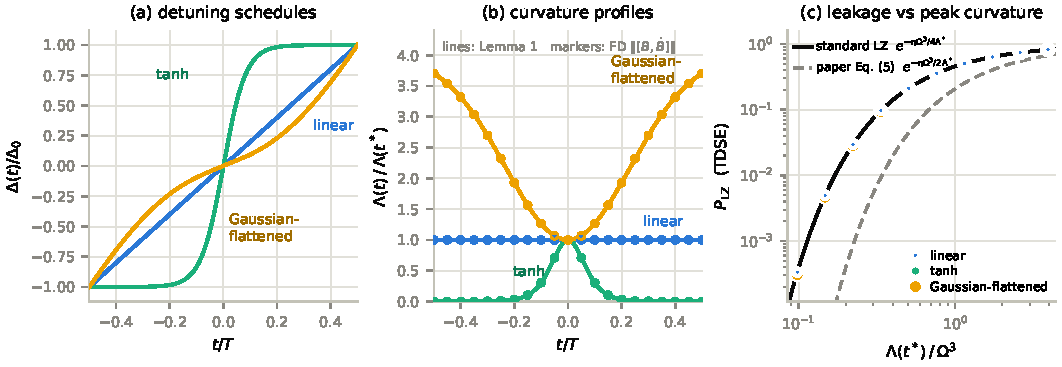
\includegraphics[width=\textwidth]{figures/fig_curvature_sweeps.pdf}
\caption{Curvature sweeps. (a)~The three detuning schedules (representative runs, $\Omega = 1$). (b)~Curvature profiles $\Lambda(t)/\Lambda(t^*)$: lines are the Lemma~1 identity $\tfrac12\Omega|\dot\Delta|$; markers are the independent finite-difference evaluation of $\|[B,\dot B]\|$ (agreement $<4\times10^{-9}$ relative). (c)~Measured leakage versus normalized peak curvature for all 90 runs (3 schedules $\times$ 3 values of $\Omega$ $\times$ 10 ramp rates; markers are nested by size because the three schedules land on the same points, and the three $\Omega$ branches coincide to $<10^{-12}$ relative---the exact scale invariance underlying the $\Lambda(t^*)/\Omega^3$ collapse). The solid curve is Eq.~\eqref{eq:lz-curvature}, $\exp(-\pi\Omega^3/4\Lambda(t^*))$, which the data follow; the dashed curve is the constant printed in earlier drafts, $\exp(-\pi\Omega^3/2\Lambda(t^*))$, retained for comparison (corrected in this revision).}
\label{fig:curvature-sweeps}
\end{figure}

%=============================================================================
\section{Discussion}
%=============================================================================

The curvature functional is a physically interpretable precursor: large $\Lambda$ indicates imminent non-adiabatic evolution. Unlike reactive control, predictive regulation of $\Lambda$ suppresses leakage before it occurs. This method extends naturally to time-varying $\Omega(t)$ and multi-qubit blocks via decomposition of $B(t)$, as derived in the authors' related patent application.

%=============================================================================
\section{Conclusion}
%=============================================================================

We introduced a spectral curvature functional that serves as a predictive control parameter for non-adiabatic transitions. For LZSM systems, $\Lambda$ yields a closed-form relationship to $P_{LZ}$, and we derive a rigorous bound on peak curvature from the spectral first moment $\int |\omega| |\hat{\Delta}(\omega)|\, d\omega$. This provides a simple control objective: minimize $\Lambda(t^*)$ and enforce $\Lambda \le \alpha_{\mathrm{crit}}$. The approach is compatible with standard waveform hardware and may be applied to semiconductor spin qubits and other electrically controlled systems.

%=============================================================================
\begin{thebibliography}{99}
%=============================================================================

\bibitem{google2023}
Google Quantum AI, ``Testing quantum error correction with real-time syndrome extraction,'' \emph{Nature}, 2023.

\bibitem{zenodo}
Zenodo Dataset: google\_105Q\_surface\_code\_d3\_d5\_d7, DOI: \url{https://zenodo.org/record/8169977}

\bibitem{landau1932}
L. D. Landau, ``On the theory of transfer of energy at collisions,'' \emph{Physikalische Zeitschrift der Sowjetunion}, vol.~2, pp.~46--51, 1932.

\bibitem{zener1932}
C. Zener, ``Non-adiabatic crossing of energy levels,'' \emph{Proceedings of the Royal Society A}, vol.~137, no.~833, pp.~696--702, 1932.

\bibitem{stueckelberg1932}
E. C. G. St\"uckelberg, ``Theory of inelastic collisions between atoms,'' \emph{Helvetica Physica Acta}, vol.~5, pp.~369--422, 1932.

\bibitem{majorana1932}
E. Majorana, ``Atomi orientati in campo magnetico variabile,'' \emph{Il Nuovo Cimento}, vol.~9, pp.~43--50, 1932.

\bibitem{doetsch1974}
G. Doetsch, \emph{Introduction to the Theory and Application of the Laplace Transformation}. Springer, 1974.

\bibitem{bracewell2000}
R. Bracewell, \emph{The Fourier Transform and Its Applications}, 3rd ed. McGraw-Hill, 2000.

\end{thebibliography}

\end{document}
